% KSN - wzór sprawozdania
% kodowanie polskich znaków: ISO-8859-2

\documentclass[10pt,a4paper]{article}
\usepackage[margin=2cm]{geometry}
\usepackage{graphicx}
\usepackage[utf8]{inputenc}
\usepackage[polish]{babel}
\usepackage{polski}
\usepackage{amsmath}
\usepackage{mathtools}
\usepackage{subcaption}
\usepackage{float}
\author{Ryniak}

\begin{document}

% =====  STRONA TYTULOWA PRACY INŻYNIERSKIEJ ====
% ostatnia modyfikacja: 2011/03/09, K. Malarz

\thispagestyle{empty}
\vspace*{50ex}
\begin{center}
{\bf\LARGE\textsf{Sprawozdanie do projeku:}}\\
\vspace{5ex}

{\bf\huge\textsf{Wykorzystanie probabilistycznych sieci neuronowych do klasyfikacji danych o zmiennym charakterze}}\\
\vspace{54ex}

{\bf\Large\textsf{Grzegorz Ryniak, Rafał Szęszoł}}\\
\vspace{22ex}
\textsf{\bf\large\textsf{Kraków, czerwiec 2018}}
\end{center}


\newpage

\section{Wstęp}
W świecie rzeczywistym często spotykamy się ze źródłami informacji, które z czasem zaczynają przesyłać zmodyfikowane dane. Przykładem może być elektroniczny czujnik grubości - odpowiednik czujnika zegarkowego. W skutek zużycia np. końcówek pomiarowych, z czasem otrzymywane wartości mogą być zaniżone. Duży problem pojawia się kiedy odbierane dane poddawane są klasyfikacji. Klasyfikator widząc przesunięcie danych może uznać, że należą one do innej klasy. Z czasem tych klas mogło by powstać coraz więcej. Ze względu na ograniczone zasoby i łatwość interpretacji często wymaga się, aby liczba klas była stała. Celem tego projektu było stworzenie klasyfikatora opartego o probabilistyczne sieci neuronowe, który byłby w stanie na bieżąco dostosowywać się do zmiennych danych. 

\section{Doświadczenia}
Wszystkie symulacje zostały przeprowadzone z wykorzystaniem środowiska MATLAB 2012b. W pierwszej kolejności stworzono generator danych, który symulował by rzeczywiste źródło informacji podlegające zużyciu. Generowane były 2 klasy dwu-wymiarowych danych. Dane takie łatwo da się przedstawić na układzie współrzędnych w postaci punktów. Pierwsza klasa składała się z punktów o współrzędnych generowanych z rozkładu Gaussa o średniej wartości (0;0) i odchyleniu 1, natomiast druga klasa również była generowana na podstawie rozkładu Gaussa o średnim odchyleniu 1 ale średnie wartości były punktami leżącymi na okręgu o promieniu 2 i środku w punkcie (0;0). Kąt pomiędzy osią x a promieniem zwiększał się z czasem w kierunku przeciwnym do wskazówek zegara. Co 90 stopni ruch na chwilę się zatrzymywał, aby sprawdzić, czy sieć nie przyzwyczaiła się do ruchu. Generowanie danych kończy się w momencie kiedy druga klasa ,,okrąży'' pierwszą dookoła. Kolejne etapy generowania danych pokazane są na rysunku \ref{dataGen}. 
\begin{figure}[h]
  \begin{subfigure}[b]{0.4\textwidth}
    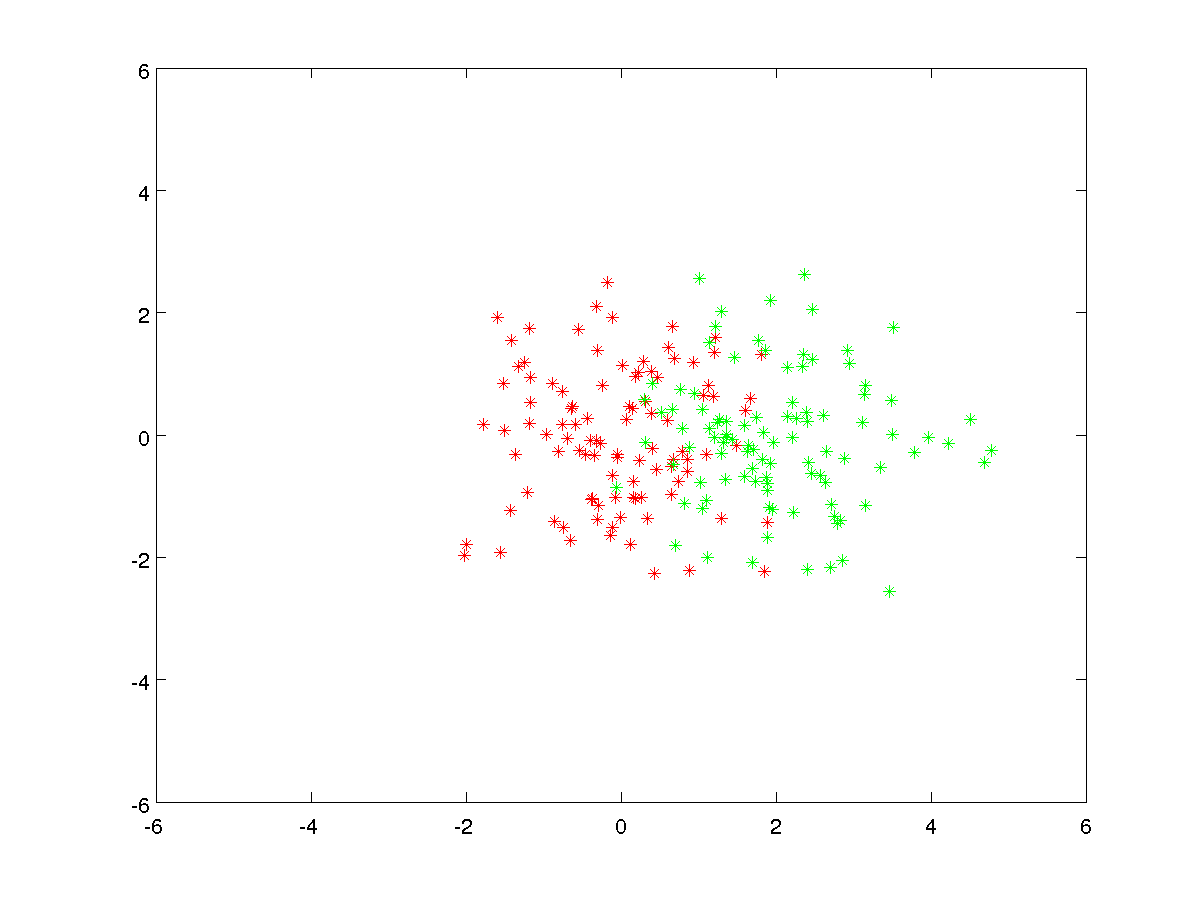
\includegraphics[width=\textwidth]{dataGen_step0.png}
    \caption{Krok 1}
  \end{subfigure}
  \hfill
  \begin{subfigure}[b]{0.4\textwidth}
    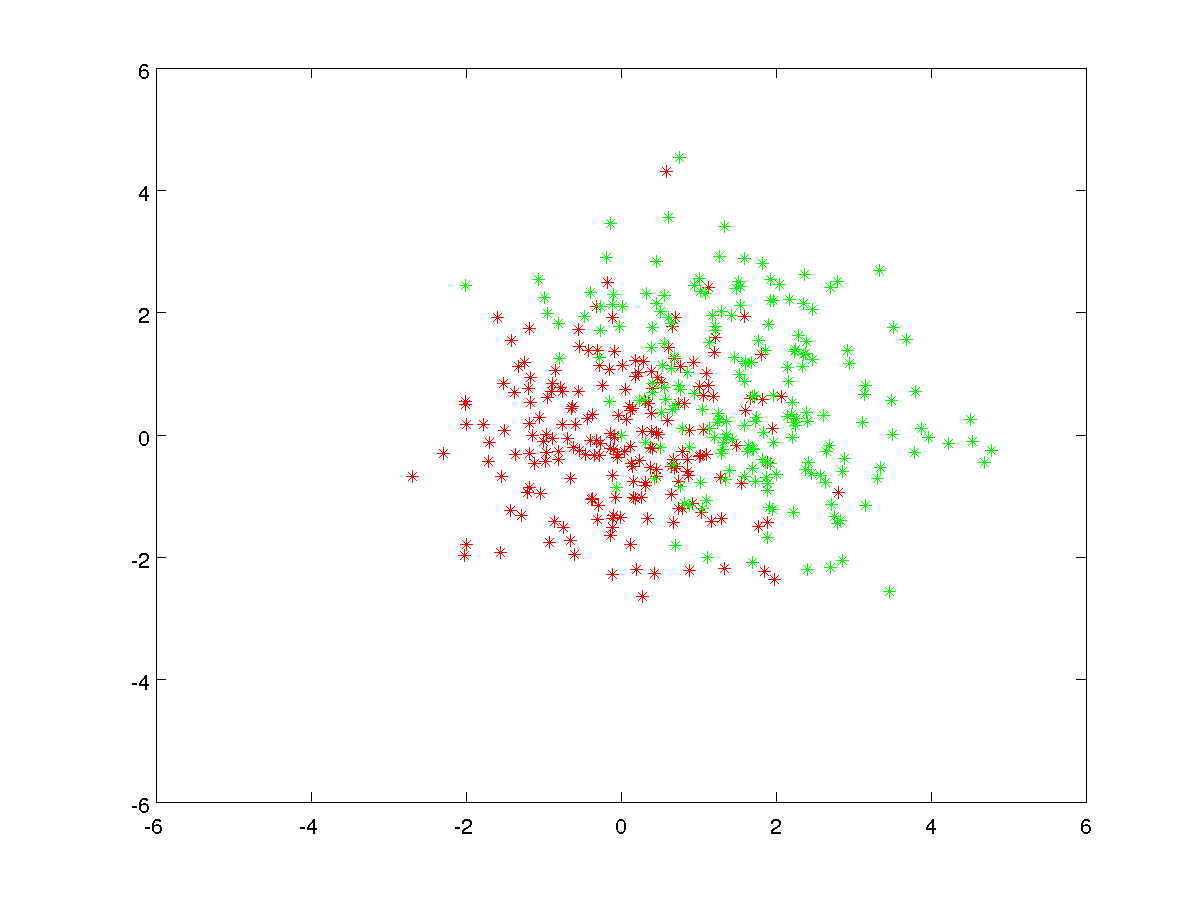
\includegraphics[width=\textwidth]{dataGen_step1.png}
    \caption{Krok 2}
  \end{subfigure}

   \begin{subfigure}[b]{0.4\textwidth}
    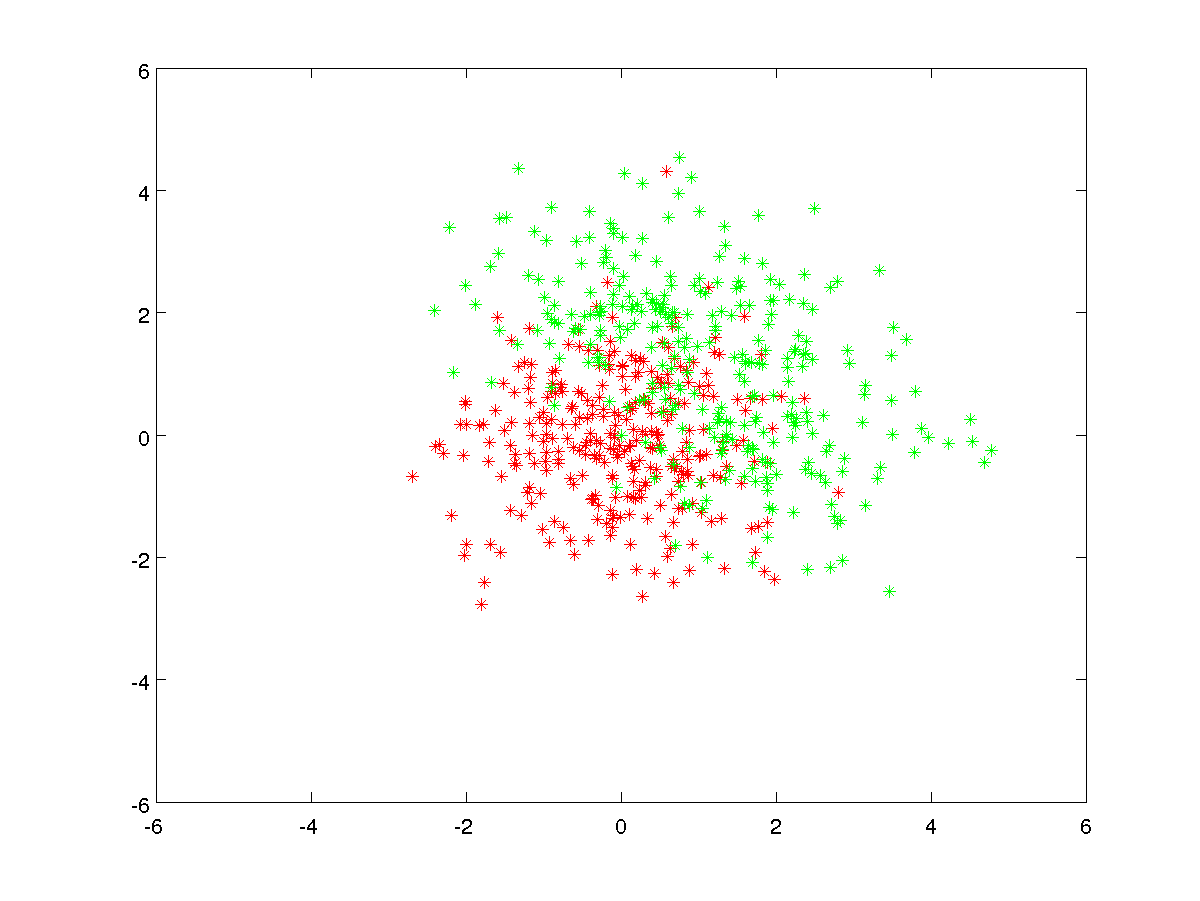
\includegraphics[width=\textwidth]{dataGen_step2.png}
    \caption{Krok 3}
  \end{subfigure}
  \hfill
  \begin{subfigure}[b]{0.4\textwidth}
    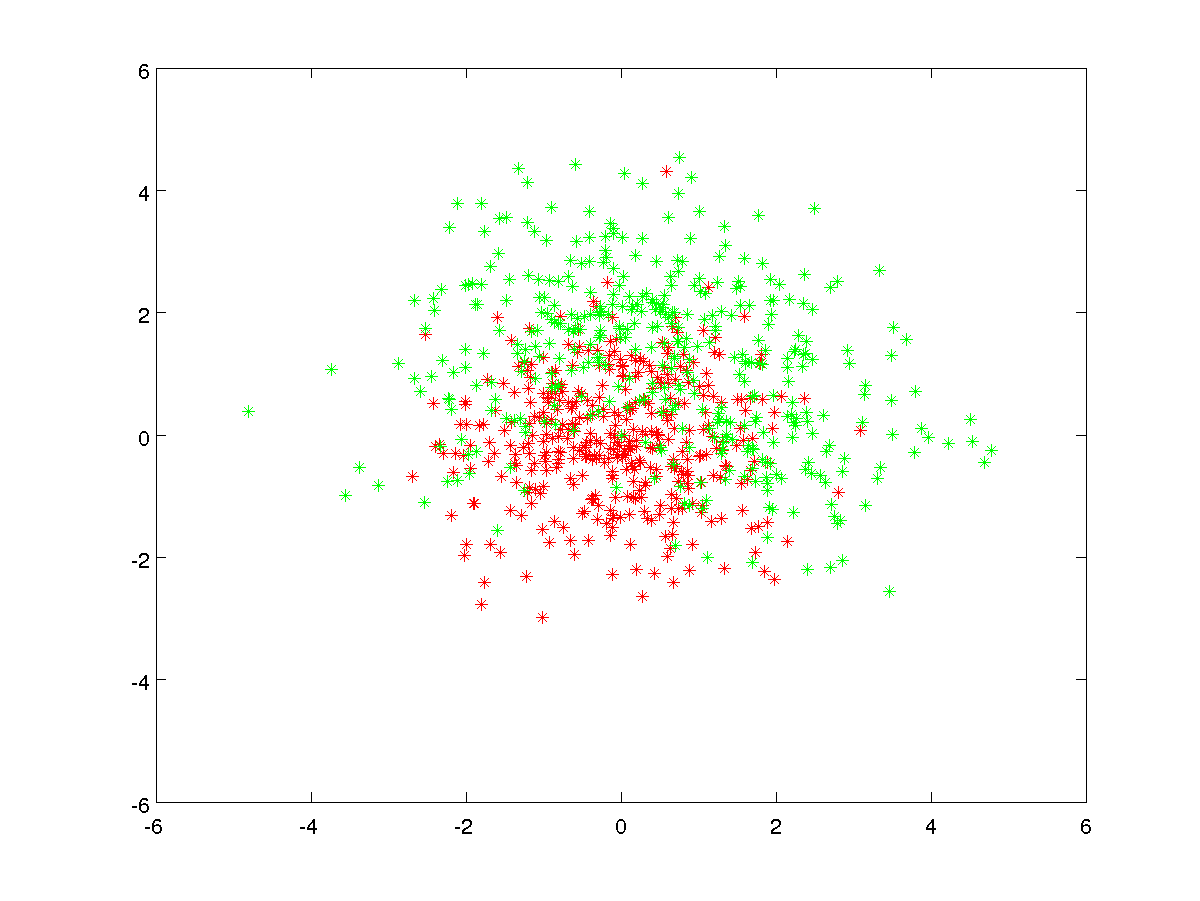
\includegraphics[width=\textwidth]{dataGen_step3.png}
    \caption{Krok 4}
  \end{subfigure}
  
  \begin{subfigure}[b]{0.4\textwidth}
    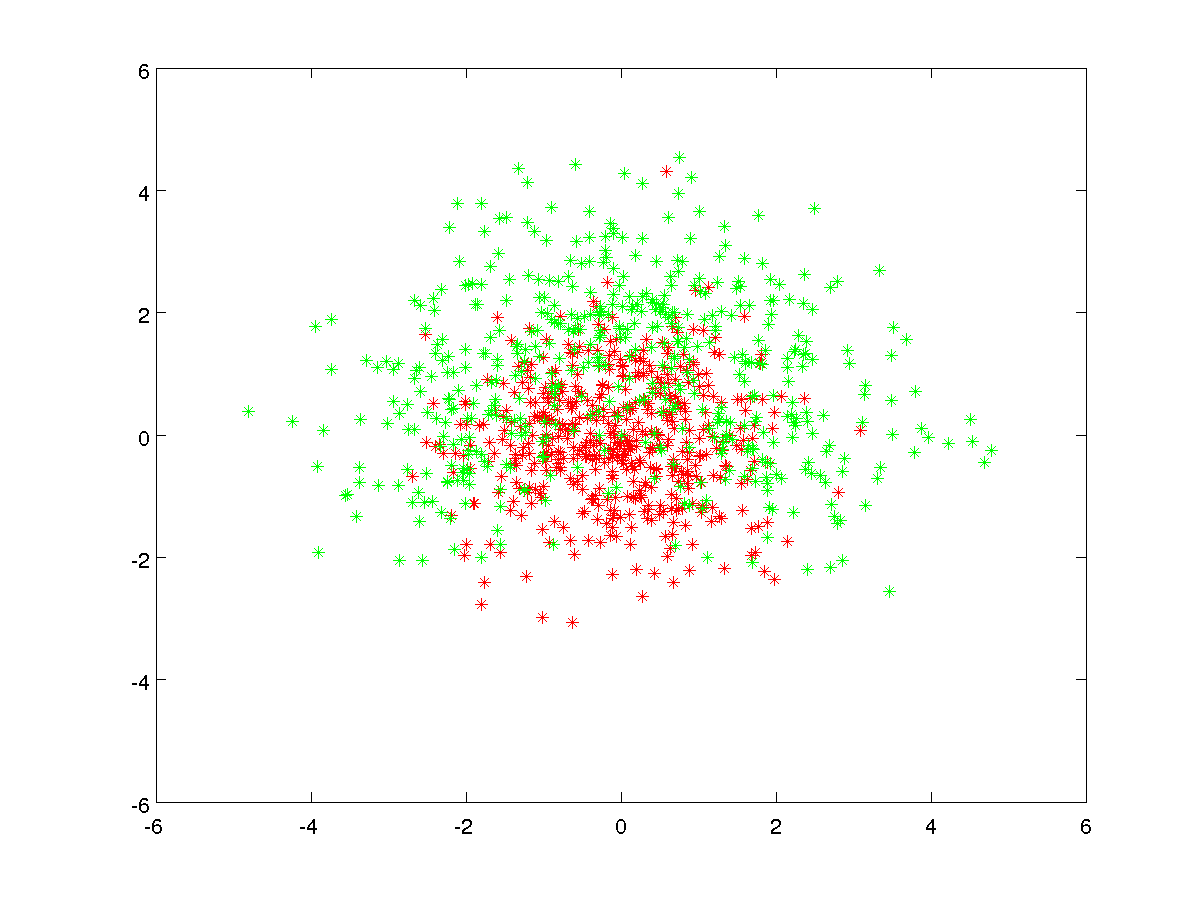
\includegraphics[width=\textwidth]{dataGen_step4.png}
    \caption{Krok 5}
  \end{subfigure}
  \hfill
  \begin{subfigure}[b]{0.4\textwidth}
    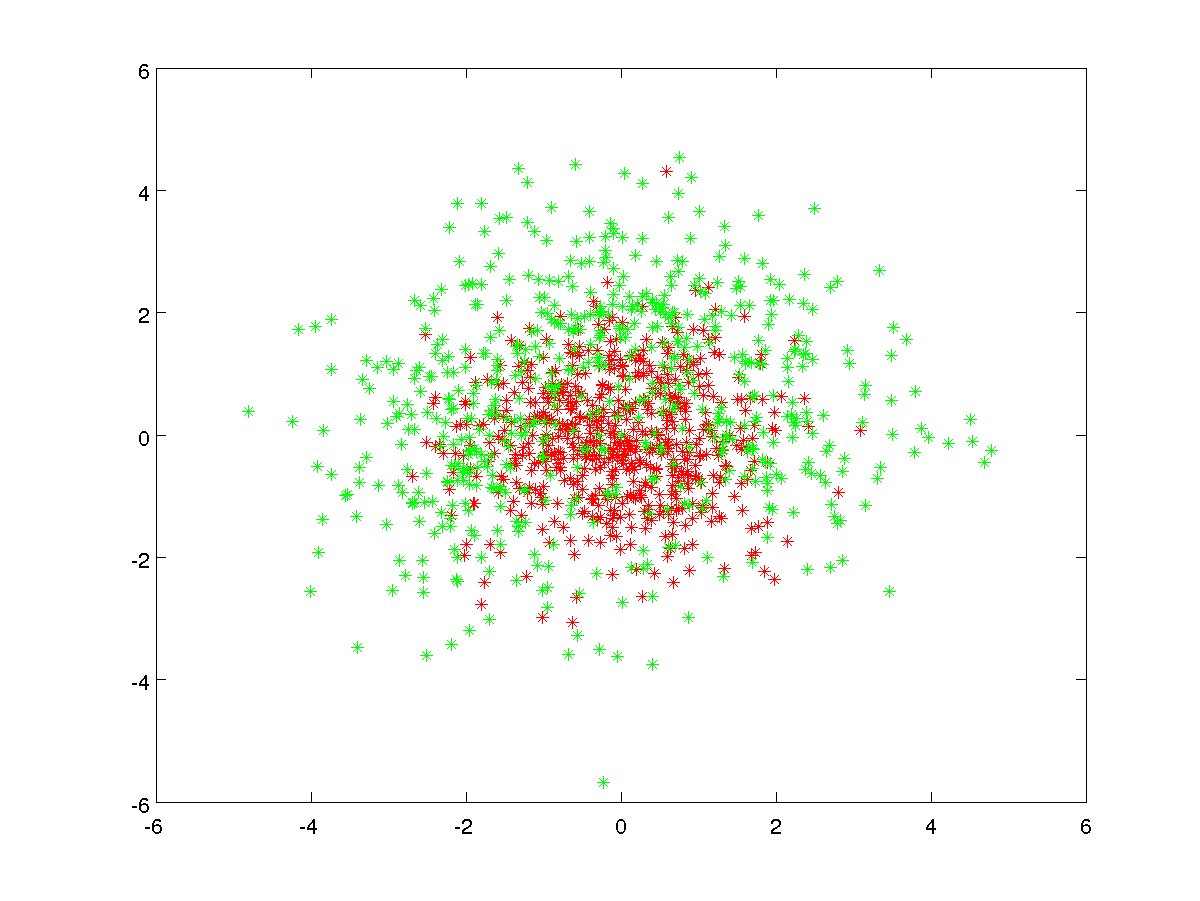
\includegraphics[width=\textwidth]{dataGen_step5.png}
    \caption{Krok 6}
  \end{subfigure}
  
  \begin{center}
  \begin{subfigure}[b]{0.4\textwidth}
    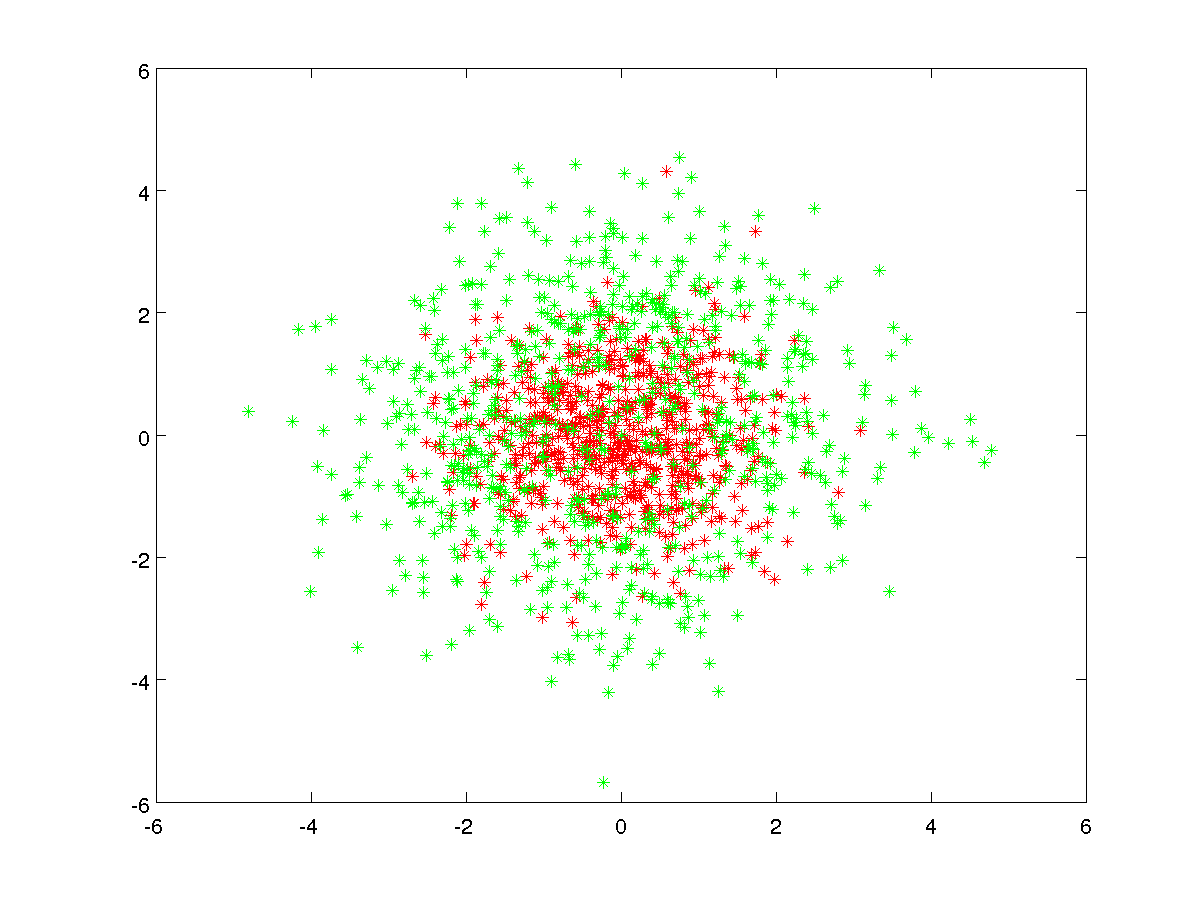
\includegraphics[width=\textwidth]{dataGen_step6.png}
    \caption{Krok 7}
  \end{subfigure}
  \end{center}
  
  \caption{Poszczególne etapy generowania danych}
  \label{dataGen}
  
\end{figure}
Liczbę punktów generowanych w każdym kroku można było zmieniać. Co określoną ilość dodanych punktów sieć neuronowa była uczona nowych danych. Dane, na których uczyła się sieć znajdowały się w kolejce. Kiedy do kolejki wchodził nowy punkt, najstarszy zostawał z niej usuwany. Długość kolejki mogła być regulowana. Podczas ponownego uczenia sieci, zmianom podlegał parametr wygładzania. Algorytm wyznaczania tegoż parametru został dostarczony przez prowadzącego zajęcia. Podczas symulacji wykonywany był wykres jak w czasie zmienia się procent błędnie sklasyfikowanych punktów oraz mapa, gdzie te punkty się znajdowały. Wartość błędu była ułamkiem wyrażonym w procentach oznaczającym ilość błędnych klasyfikacji w obrębie całego okna na ilość dodanych nowych punktów, zatem wartość ta może przekroczyć 100 \%. 

Na początku przeprowadzono testy dla stałego parametru wygładzania (wartość spread). Liczbę wszystkich generowanych punktów ustawiono na 8000, natomiast aktualizacja sieci odbywała się co 50 punktów. Rozmiar okna wynosił 1000 punktów. Symulacje przeprowadzono dla spread równego 0,0001; 0,001; 0,01; 0,1 oraz 1. Dla każdego testu sporządzona został mapa z błędnymi punktami w ostatniej fazie, wykres zależności błędu od czasu oraz średnia wartość błędu. Wyniki przedstawia rysunek \ref{test_h} oraz tabela \ref{h_table}.

\begin{figure}[h]
  \begin{subfigure}[b]{0.5\textwidth}
    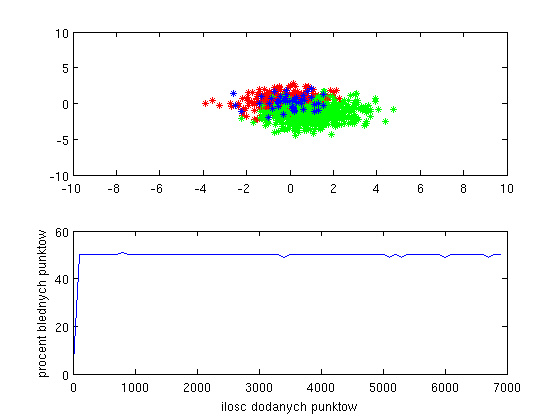
\includegraphics[width=\textwidth]{test_h0_0001.png}
    \caption{h = 0,0001}
  \end{subfigure}
  \hfill
  \begin{subfigure}[b]{0.5\textwidth}
    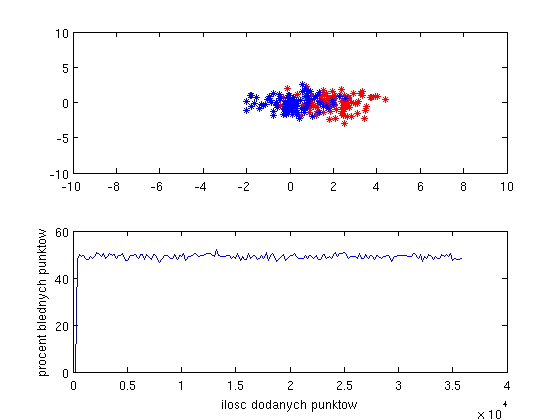
\includegraphics[width=\textwidth]{test_h0_001.png}
    \caption{h = 0,001}
  \end{subfigure}

   \begin{subfigure}[b]{0.5\textwidth}
    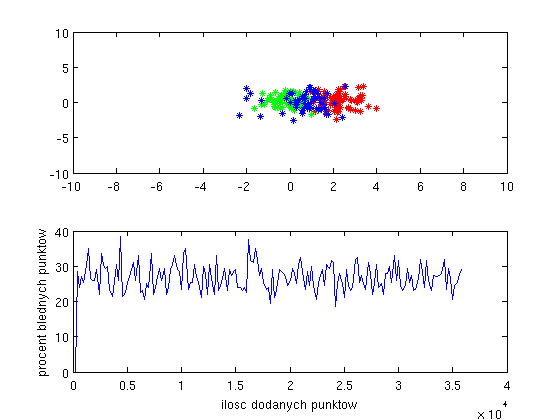
\includegraphics[width=\textwidth]{test_h0_01.png}
    \caption{h = 0,01}
  \end{subfigure}
  \hfill
  \begin{subfigure}[b]{0.5\textwidth}
    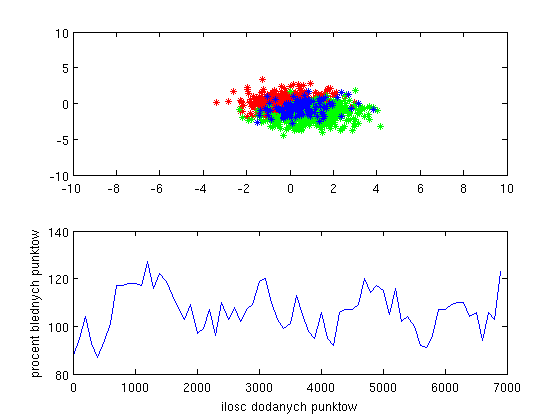
\includegraphics[width=\textwidth]{test_h0_1.png}
    \caption{h = 0,1}
  \end{subfigure}
  
  \begin{center}
  \begin{subfigure}[b]{0.5\textwidth}
    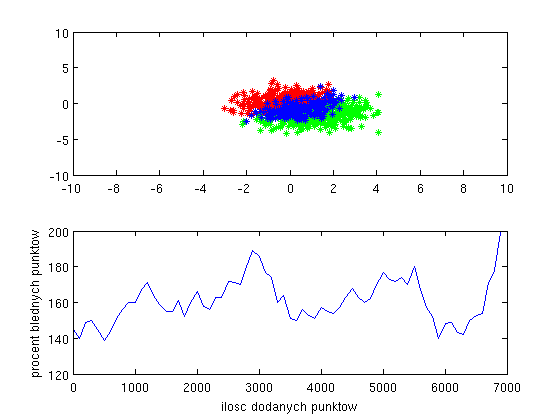
\includegraphics[width=\textwidth]{test_h1.png}
    \caption{h = 1}
  \end{subfigure}
  \end{center}
  
  \caption{Poszczególne etapy generowania danych}
  \label{test_h}
  
\end{figure}

\begin{table}[H]
\centering
\begin{tabular}{|c|c|}
\hline
spread & błąd \\
\hline
0,0001 & 50\%  \\
\hline
0,001 & 45\%  \\
\hline
0,01 & 25\%  \\
\hline
0,1 & 106\%  \\
\hline
1 & 160\%  \\
\hline
\end{tabular}
\caption{Zestawienie wyników testów dla stałych wartości spread.}
\label{h_table}
\end{table}
Następnie przeprowadzono symulację dla h - wartości spread liczonej automatycznie. 

Parametry danych były jak w poprzednim przypadku. Rysunek \ref{test_h_auto} przedstawia otrzymane wyniki. Sporządzone wyniki zostały uzupełnione o wartość współczynnika wygładzenia zmieniającego się w czasie. 

\begin{figure}[h]
\centering
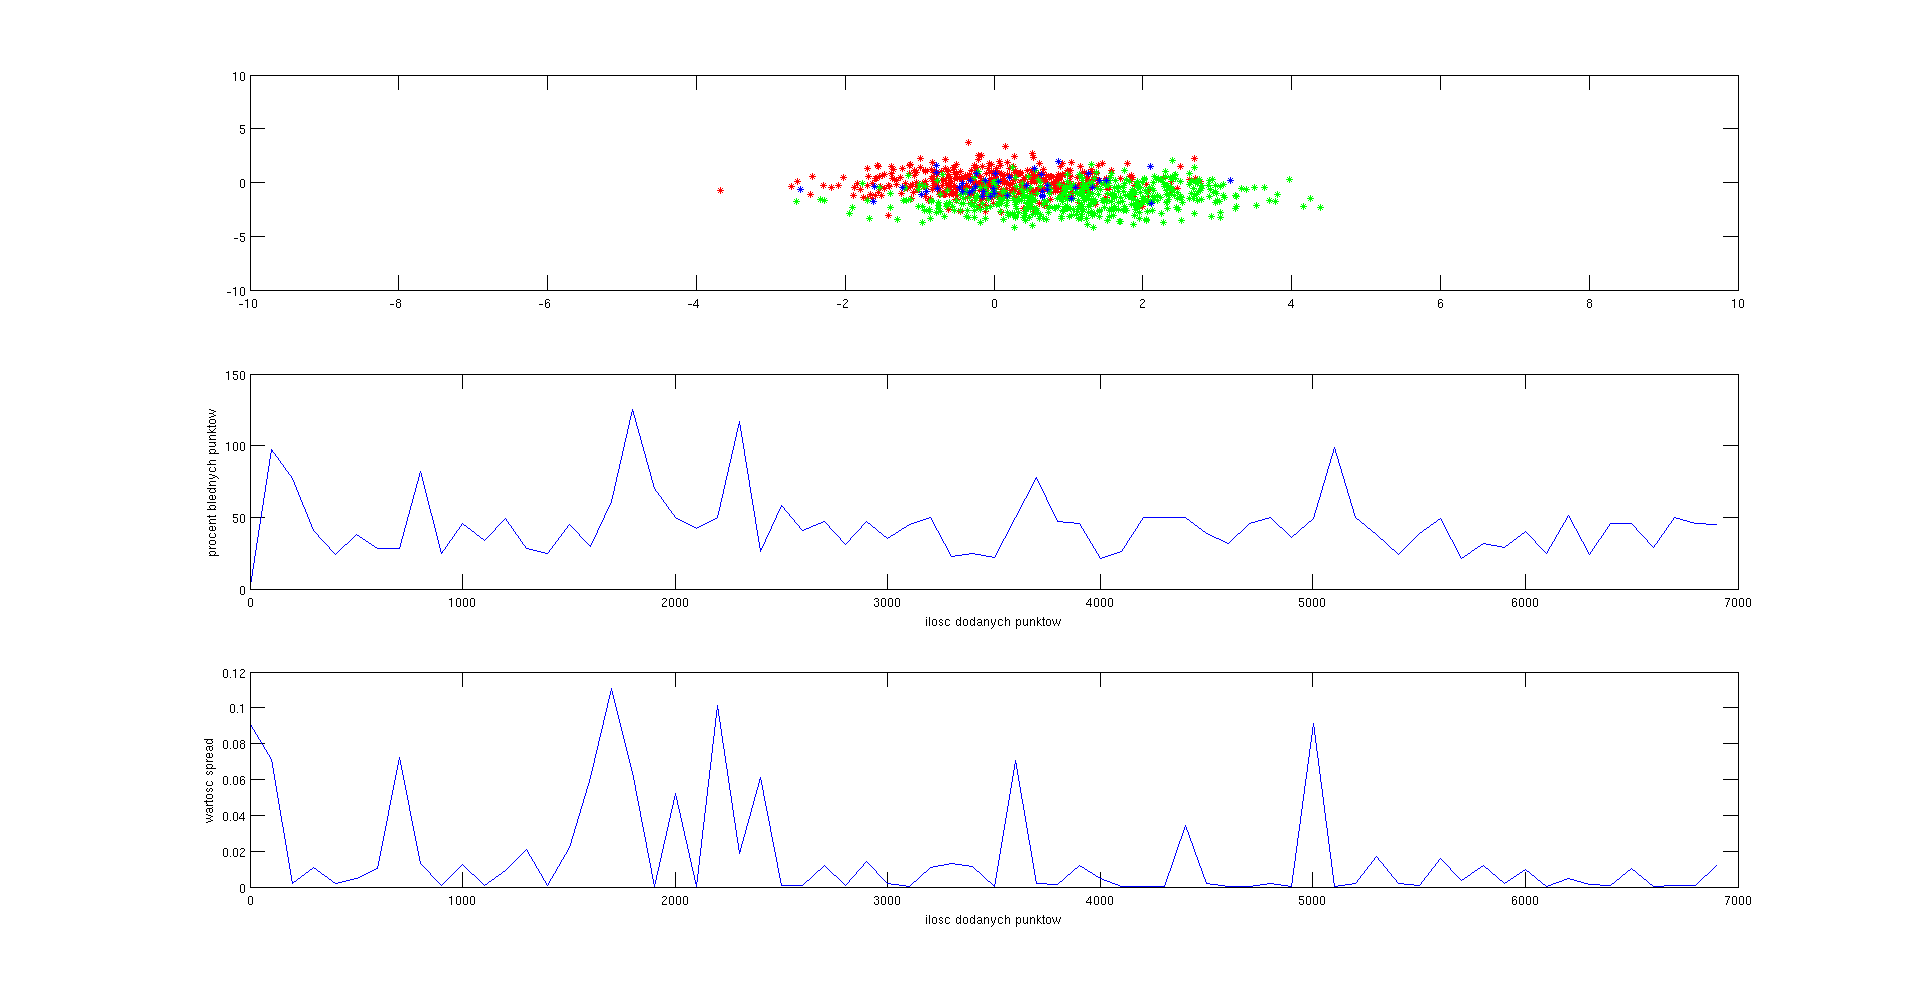
\includegraphics[width=15cm]{test_h_auto.png}
\caption{Symulacja dla spread liczonego automatycznie.}
\label{poj}
\end{figure}

Średni błąd wyniósł 40 \%. 


\section{Wnioski}
Spoglądając na wyniki dla różnych wartości spread można zauważyć ciekawe zjawiska. Dla bardzo małej wartości błąd utrzymywał się na poziomie 50\%. Wynika to z faktu, że sieć rozpoznawała tylko punkty nauczone w poprzedniej iteracji, gdyż zasięg funkcji bazowej był praktycznie zerowy. W miarę zwiększania parametru wygładzania, błąd się zmniejszał, by osiągnąć minimalną wartość dla spread równego 0,01. Kiedy wartość była dalej zwiększana, błąd rósł ponad 100 \% ponieważ zasięg funkcji bazowych był tak duży, że nawet punkty wyuczone w poprzedniej iteracji były błędnie klasyfikowane. W czasie trwania symulacji nie zauważono znaczącego wpływu przemieszczania się punktów drugiej klasy na błędne sklasyfikowane punkty. 

Symulacja z automatycznym liczeniem współczynnika wygładzania działa gorzej niż dla niektórych wartości ustawionych na sztywno. Powodem tego mogło być wadliwe działanie metody Q(0) dla wariantu PNNS. W pewnych warunkach algorytm tracił stabilność i sztucznie zawyżał wartości spread.  


\end{document}